

\documentclass[11pt,a4paper,titlepage,oneside]{article}

\usepackage[most]{tcolorbox}
\usepackage{geometry}
\usepackage{svg}

\usepackage{setspace}

\usepackage{titlesec} % skip after \section

\usepackage{hyperref} %links
\usepackage{xurl}

\usepackage[document]{ragged2e} %floating text
\usepackage{helvet} %font
\usepackage{tocloft} % dots in table of contents sections

\usepackage{lipsum, multicol}
\usepackage{fancyhdr}
\usepackage{listings}

\usepackage{array}

\usepackage{pdfpages}


% citaitons
\usepackage{natbib}

% hypthenationrules
\usepackage[T1]{fontenc}



%redefine the entire fucking bib environment so we dont have the horisontal spacing
% this was generated entirely by chatgpt

\makeatletter
\renewenvironment{thebibliography}[1]
  {\section{Lähteet}%
   \@mkboth{\MakeUppercase{\refname}}{\MakeUppercase{\refname}}%
   \list{\@biblabel{\@arabic\c@enumiv}}%
        {\settowidth\labelwidth{\@biblabel{#1}}%
         \leftmargin\labelwidth
         \advance\leftmargin\labelsep
         \setlength\itemindent{-\labelwidth}
         \setlength\itemsep{10pt} % Change this value to adjust the space between items
         \@openbib@code
         \usecounter{enumiv}%
         \let\p@enumiv\@empty
         \renewcommand\theenumiv{\@arabic\c@enumiv}}%
   \sloppy
   \clubpenalty4000
   \@clubpenalty \clubpenalty
   \widowpenalty4000%
   \sfcode`\.\@m}
  {\def\@noitemerr
    {\@latex@warning{Empty `thebibliography' environment}}%
   \endlist}
\makeatother





%this is such a shitshow lmao

\hypersetup{
    colorlinks=false,
    citecolor=black,
    filecolor=black,
    linkcolor=black,
    linkbordercolor=1 1 1,
    citebordercolor=1 1 1,
    pdfborderstyle={/S/U/W 1},
    urlbordercolor=0 0 1,
    urlcolor=blue
}
\urlstyle{same}



\geometry{
    a4paper,
    left=3cm,
    right=2.5cm,
    top=3cm,
    bottom=2.5cm
}

%remove random margin on side ? idk what happend
%\setlength{\oddsidemargin}{0pt}


%these need to be overridden in coverpage
\renewcommand{\baselinestretch}{1.5} 
\setlength{\parskip}{0.1cm}


%custom reusable colorbox rules
\newtcolorbox{simplebox}{colback=white, sharp corners, boxrule=1pt }


\renewcommand{\contentsname}{Sisällys} % override Contents => Sisallys on table of contents
\renewcommand{\cftsecpagefont}{\normalfont} %remove section bold font in toc
\renewcommand{\cftsecfont}{\normalfont}% remove section bold font in toc
\setlength{\cftbeforesecskip}{0px} % remove weird vfill between toc sections


\renewcommand{\familydefault}{\sfdefault} % set font

\renewcommand{\cftsecleader}{\cftdotfill{\cftdotsep}} % dots for sections

\renewcommand{\bibsection}{\section{Lähteet}} % bibbliio name on lähteet sectio

\setlength{\headheight}{13.6pt}

%space after the sections
% ?, before, after
\titlespacing{\subsection}{0pt}{0.5cm}{0.5cm}

\def\filename{src/oppari.tex}





%\def\testmode{1}




\newcommand\wordcount{
    \immediate\write18{texcount -sub=section \filename{} -inc  | grep Section | sed -e 's/+.*//' | sed -n \thesection p > 'count.txt'}
(\input{count.txt}words)}


\newcommand{\inputf}[1]{\def\filename{#1}\input{#1}}


\newcommand\filewcount{
    \immediate\write18{texcount -1 -sum \filename{} > count.txt }
    \input{count.txt} words }


% jos on testi definetty niin tee 
\newcommand{\istest}[2]{\ifx\testmode\undefined #2 \else #1 \fi}


% testi section näyttää word countin siltä sectionilta jos ei testi niin sitten näytä vain normaali section
\newcommand{\tsection}[2]{\istest{#1{#2\\} \wordcount \\ \medskip }{#1*{#2}}}


\newcommand{\pagesection}[1]{\istest{\section{#1}  }{\section*{#1}}}
\newcommand{\pagesubsection}[1]{\istest{\subsection{#1}  }{\subsection*{#1}}}


% adds page with everything
\newcommand{\addPage}[2]{
    \def\filename{#1}
    \pagesection{#2}
    \istest{ \filewcount \medskip }{}
    \input{#1}
}



% OPPARI SPESIFIC

\newcommand{\addPageOp}[2]{
    \def\filename{#1}
    \pagesubsection{#2}
    \istest{ \filewcount \medskip }{}
    \input{#1}
}

%lab citation style
\newcommand{\labcite}[1]{\setcitestyle{aysep={},open={(},close={.)}}\citep{#1}{}}

%lab citation style
\newcommand{\labciteend}[1]{\setcitestyle{aysep={},open={(},close={).}}\citep{#1}{}}

\newcommand{\labimgcite}[1]{\setcitestyle{aysep={},open={(},close={)}}\citep{#1}{}}

\newcommand{\hurl}[1]{\href{#1}{{\underline{\textcolor{blue}{#1}}}}}


% counter kuville
\newcounter{imgCounter}
\setcounter{imgCounter}{0}

\newcommand{\getImgCount}{
\addtocounter{imgCounter}{1}
\theimgCounter
}


% counter kaavioille
\newcounter{chartCounter}
\setcounter{chartCounter}{0}

\newcommand{\getChartCount}{
\addtocounter{chartCounter}{1}
\thechartCounter
}



\usepackage[finnish]{babel}








% ------------------------------ BEGIN DOCUMENT ------------------------------ %
\begin{document}

\pagestyle{empty}


%------------------------------ COVER PAGE ------------------------------ %


\includegraphics[width=5cm,height=1cm]{./src/labimg.jpg}

%override baselinestretch thing in this area
\renewcommand{\baselinestretch}{1} 
\setlength{\parskip}{0cm}

\vspace{86mm}
{\huge
\textbf{Kehittymisen seuranta web-teknologioissa:\\ MongoDb, MeteorJs ja ReactJs}
}
\newline

{\large

\vspace{5mm}
\textbf{Oppimispäiväkirja}
}

\vspace{80mm}

LAB-ammattikorkeakoulu \newline
\vspace{2mm}
Tieto-ja viestintätekniikka, Insinööri (AMK) \newline
\vspace{2mm}
2024 \newline
\vspace{2mm}
Kimi Malkamäki

\newpage




%------------------------------ ABSTRACT PAGES ------------------------------ %


\begin{spacing}{1} %\baselinestretch
    \setlength{\parskip}{0.5cm} 
    
\begin{tabular}{ | l | }

    %hack for the tiivistelmä line
    \multicolumn{1}{l}{
        \begin{minipage}{6cm}
            \hspace{1mm}
            
        \end{minipage}
        \begin{minipage}{4.25cm}
            \hspace{1mm}
        \end{minipage}
        \begin{minipage}[t][1.95cm][t]{3.62cm}
            \large
            \textbf{ Tiivistelmä }
        \end{minipage}
    }\\

    \hline
    \begin{minipage}[b]{6cm}
        Tekijä(t)
        \newline
        Kimi Malkamäki 
    \end{minipage}%
    % 2x2
    \begin{minipage}{8.5cm}
        \begin{tabular}{ | l | c | }
            \begin{minipage}[t][1cm][t]{4.25cm}
                Julkaisun laji
                \newline
                Opinnäytetyö, AMK
            \end{minipage} & %
            %
            \begin{minipage}{3.62cm}
                Valmistusaika
                \newline
                2024
            \end{minipage} \\ \hline%
            %
            \begin{minipage}[t][1cm][t]{4.25cm}
                Sivumäärä
                \newline 
                31+19
            \end{minipage}
            &  \\ \hline
        \end{tabular}
    \end{minipage}%
    % end of 2x2
      \\ \hline

    \begin{minipage}[t][2cm][t]{8cm}
    Työn nimi 
        \newline 
    ammatissa kasvaminen 
        \newline 
    oppimispäiväkirja  
    \end{minipage}\\ \hline

    \begin{minipage}[t][1.5cm][t]{10cm}
    Tutkinto ja koulutusala.\newline  Tieto- ja viestintätekniikka, insinööri AMK  

    \end{minipage}\\ \hline

    \begin{minipage}[t][7.5cm][t]{14.5cm}
    Tiivistelmä: \medskip 
    
    Opinnäitettyön tavoitteena oli seurata ammattimaista kehittymistä 13 viikon seurantajakson aikana, 
        jolloin kirjoitettiin oppimispäiväkirja. Päiväkirjaan on kirjattu haasteet ja ongelmat, mihin törmäsin harjoittelun aikana. \medskip

    Työtehtäviini seurantajakson aikana kuului 
        ominaisuuksien suunnittelu ja toteutus web alustaan ja sovelluksen ohjelmavirheiden korjaukset.
        Ominausuuksien toteuttamisessa ja sen prosessin dokumentoimisessa oppimispäiväkirjaan antaa hyvän silmäyksen alan ammattilaisen arkipäiväiseen työhön 
        ja haasteisiin mitkä ilmeentyvät päivittäin. \medskip

    Olen selvästi parantanut sosiaalisia ja teknisiä taitojani tämän kokemuksen myötä.
        Saamastani käytännön työkokemuksesta on epäilemättä hyötyä tulevalla urallani.
        Päiväkirjan avulla olen voinut pohtia edistymistäni ja tunnistaa alueita, joilla voin edelleen kehittyä. 

    \end{minipage}\\ \hline

    \begin{minipage}[t][2cm][t]{14cm}
    Avain sanat \medskip

    MeteorJS, ReactJs, MongoDB, Web suunnittelu, Responsiivinen suunnittelu
    \end{minipage}\\ \hline

\end{tabular}


\newpage

% ------------------------------ SECOND PAGE OF ABSTRACT ------------------------------ %

\begin{tabular}{ | l | }

    %hack for the tiivistelmä line
    \multicolumn{1}{l}{
        \begin{minipage}{6cm}
            \hspace{1mm}
            
        \end{minipage}
        \begin{minipage}{4.25cm}
            \hspace{1mm}
        \end{minipage}
        \begin{minipage}[t][1.95cm][t]{3.62cm}
            \large
            \textbf{ Abstract }
        \end{minipage}
    }\\

    \hline
    \begin{minipage}[b]{6cm}
        Author(s)
        \newline
        Kimi Malkamäki 
    \end{minipage}%
    % 2x2
    \begin{minipage}{8.5cm}
        \begin{tabular}{ | l | c | }
            \begin{minipage}[t][1cm][t]{4.25cm}
                Type of Publication 
                \newline
                Thesis, UAS?
            \end{minipage} & %
            %
            \begin{minipage}{3.62cm}
                Published
                \newline
                2024
            \end{minipage} \\ \hline%
            %
            \begin{minipage}[t][1cm][t]{4.25cm}
                Number of Pages
                \newline 
                31+50
            \end{minipage}
            &  \\ \hline
        \end{tabular}
    \end{minipage}%
    % end of 2x2
      \\ \hline

    \begin{minipage}[t][2cm][t]{8cm}
    Title of Publication
        \newline 
    ammatissa kasvaminen 
        \newline 
    oppimispäiväkirja  
    \end{minipage}\\ \hline

    \begin{minipage}[t][1.5cm][t]{10cm}
    Degree, Field of Stydy.\newline  Bachelof of information and communication Technologies

    \end{minipage}\\ \hline

    \begin{minipage}[t][7.5cm][t]{14.5cm}
    Abstract: \medskip 

    The objective of the study was to observe and document my professional development over a 13-week follow-up period.
        This was achieved by maintaining a learning diary, 
        in which i recorded the challenges and problems encountered during their training. \medskip

    The follow-up period entailed the design and implementation of new features for the web platform,
        as well as the resolution of technical issues within the application.
        The implementation of features and the subsequent documentation of the process in a learning diary provides insight into the daily work of a professional in the field and the challenges that they encounter on a daily basis. \medskip

    % not evident
    It is clear that this experiance has notably improved my social and technical abilities. 
        The practical work experience I have gained will prove advantageous in my future career.
        The diary has given me the chance to reflect on my progress and identify areas where i require further improvement.

    \end{minipage}\\ \hline

    \begin{minipage}[t][2cm][t]{14cm}
        Keywords
        \medskip

        MeteorJS, ReactJs, MongoDB, Web design, Responsive design 
    \end{minipage}\\ \hline

\end{tabular}

\end{spacing}



\newpage


% ------------------------------ TABLE OF CONTENTS ------------------------------ %


%keep page numbers off
\setcounter{page}{0}
\pagestyle{empty}
\pagenumbering{gobble}

\tableofcontents





\newpage



% ------------------------------- TERMISTÖ ------------------------------- %

\textbf{ TERMISTÖ }\\
\bigskip

\begin{tabular}{ p{3.7cm} b{12cm} }
ECMAscript\bigskip & Skriptaus-kieli standardi \\ 
Client\bigskip & Asiakasohjelma\\
DOM\bigskip & Document Object Model\\
VDOM\bigskip & Virtual DOM\\
Transpilaatio\bigskip & Ohjelmointikielen kääntäminen toiseen ohjelmointikieleen\\
CSS\bigskip & Cascading Style Sheets\\
HTML\bigskip & Hypertext Markup Language\\
JSX\bigskip & JavaScript syntaksi jatke\\
JSON\bigskip & JavaScript Object Notation\\
NoSql\bigskip & Ei relatiivinen tietokantajärjestelmä\\
Front-end\bigskip & Sovelluksen ulkonäköä määritävä koodi\\
Full-stack\bigskip & Koko sovellusta kattava koodi\\
RPC\bigskip & Remote Procedure Call\\
REST\bigskip & Representional state transfer\\
NPM\bigskip & Node package manager\\
\end{tabular}




\newpage

% ------------------------------- CONTENT PRELUDE COMMANDS ------------------------------- %
%enable page counting
\pagenumbering{arabic}
\clearpage
\setcounter{page}{1}

%set heaader and footer
\pagestyle{fancy}
%%
\lfoot{}
\cfoot{}
\rfoot{}
%%
\lhead{}
\chead{}
\rhead{\thepage}
%%
\renewcommand{\headrulewidth}{0pt}
\renewcommand{\footrulewidth}{0pt}


%\newcommand{\n}{\newline\vspace{20mm}}





    






\section{Johdanto}              % ------------------------------- JOHDANTO ------------------------------- %



% jotain joko lähde tai muukkaa sanoitus ettei se ole väite

Teknologia-ala on nopealiikkeinen ja dynaaminen. 
Uusia teknologioita ja innovaatioita syntyy jatkuvasti, kun taas vanhat poistuvat nopeasti käytöstä.
Alan ammattilaisten on pysyttävä valppaana ja osallistuttava jatkuvasti aktiiviseen oppimiseen ja taitojen kehittämiseen,
jotta he pysyvät mukana alan uusimmista edistysaskelista ja suuntauksista.\labcite{vitaly18}
\medskip




Opinnäytetyö on kirjoitettu päiväkirjamuodossa. 
Ennen opinnäytetyön kirjoittamisen aloittamista oli 13 viikon seurantajakso, jonka aikana kirjoitin teknologioista,
joiden kanssa työskentelin, sekä muistiinpanoja toiminnastani ja oppimiskokemuksistani.
Tämä päiväkirja on katsaus tieto- ja viestintätekniikan alan ohjelmistokehittäjän päivittäiseen työhön,
ja se antaa käsityksen niistä lukemattomista haasteista, joita alalla päivittäin kohdataan.
Se kuvaa ongelmanratkaisun, projektinhallinnan ja jatkuvan täydennyskoulutuksen tarvetta.
Seurantajakson aikana syvennyin minulle uusien teknologioiden ja web-alustojen kehittämisen oppimiseen ja sain näkemyksiä ja käytännön tietoa,
jotka paransivat merkittävästi ammatillista osaamistani.
\medskip



% 
Opinnäytettyön tavoitteena on seurata kehitymistä ja teknologoiden oppimista seurantajakson aikana.
% 
Oppimispäiväkirja on kirjoitettu teemoittain teknologioista, joita käytin ja opiskelin seurantajakson aikana.
Teemat voivat kattaa useamman viikon ja niissä kerrotaan itse teknologioista. 
Teemoissa myös kerrotaan miten käytin kyseistä teknologiaa viikon tehtävien toteuttamiseen ja
ongelmiin, joihin törmäsin niitä käyttäessäni.
\medskip




%selitys starttaamosta ja mistä se tekee/haluaa


Opinnäytetyö toteutettiin Starttaamo Oy:ssä. Starttaamo Oy on suomalainen startup-yritys,
 joka pyrkii rakentamaan web-alustan yrityksille kokonaisvaltaisen hyvinvoinnin ratkaisemiseen.
%
%Startupin pää tavoitteena on vähentää sairaslomia saamalla työntekijät noudattamaan, alojen ammattilaisten suunnittelemien liikunta- ja ruokavalio-ohjelmia. 
% 
%
Olin mukana web-alustan kehittämisessä, jossa
%Yrityksen pää myyntituote on web-alusta, jonka kehittämisessä olin mukana. 
%
%Alustan kehittämisessä 
sain mahdollisuuden työskennellä tuotantoympäristössä ja minulle uusien teknologioiden kanssa.
Olin mukana suunnittelussa, ominaisuuksien lisäämisessä ja ohjelmoinnissa. 
Sain myös kokemusta ongelmien korjaamisesta.

%more
\medskip










\newpage
\section{Lähtötilanne}         % ------------------------------- LÄHTÖTILANNE ------------------------------- %




Ennen opinnäytetyön kirjoittamista ja seurantajakson alkamista olin opiskellut LAB-\\ammattikorkeakoulussa 7 lukukautta ja
olin opinnäytetyön kirjoituksen aikana neljännen vuoden tieto- ja viestintätekniikan opiskelija.
Vaikka minulla ei ollut aiempaa työkokemusta tieto- ja viestintätekniikan alalta ennen harjoituksen alkamista,
olin koulutuksen aikana saanut laajan pohjan ohjelmoinnista,
sen perusteista ja muista tieto- ja viestintätekniikan alan taidoista esim. versionhallinnasta, tietokannoista sekä web-suunnittelusta.
Teoriapohja ei kuitenkaan aina riitä työelämässä, joten uusiin olosuhteisiin sopeutuminen ja uusien asioiden oppiminen on oleellista.
\medskip




Harjoittelun aikana halusin oppia web-alustojen kanssa työskentelystä ja projektissa käytetyistä teknologioista.
Halusin myös kokemusta työskennellä muiden suunnittelemassa, suuressa koodipohjassa.
Isommat projektit vaativat palavereita ja yhteenvetoja, jotta kaikki kehittäjät pysyvät ajan tasalla.
Koska minulla ei ole aiempaa työkokemusta, minulla on puutteita ammatillisissa sosiaalisissa taidoissa.
%
Viikottaisiin palavereihin osallistuminen ja viikon aikana tehtyjen töiden esittely 
ja selittäminen on oleellinen taito ammatillisessa työelämässä, minkä halusin oppia.
\medskip


Web-sovelluksen kehittämisessä tulee esiin haasteita, joita ei tule muussa sovelluskehityksessä.
Sovellukset koostuvat useimmiten monesta osasta, kuten front-end, back-end ja tietokanta.
% 
Sovelluksen toiminnan kannalta kaikkien näiden osien pitää olla jatkuvasti yhteyksissä toisiinsa, ja niiden katkeaminen 
voi johtaa sovelluksen toimimattomuuteen.
Myös palvelin- tai muut sovellusvirheet voivat kaataa sovelluksen kaikilta käyttäjiltä. 
Web-sovelluksien kehittämisessä on myös etuja tavalliseen sovelluskehitykseen verrattuna, kuten 
web-sovelluksen päivityksen saanti käyttäjille on nopeaa ja kaikki käyttäjät saavat päivityksen samanaikaisesti.
\medskip

Harjoituksen aika työskentelin Startupin web-alustan kanssa. 
Olin mukana sen kehityksessä, suunnittelussa, ominaisuuksien lisäämisessä ja sivustojen ylläpidossa.
Alusta oli käyttöönotettu ennen harjoittelun alkamista ja siellä oli aktiivisia käyttäjiä.
Alustan kehityksessä oli keskitytty kehitysnopeuteen,
joten alustalta puuttui monia ominaisuuksia, joita odotetaan web-sovelluksesta, 
kuten web-sivustojen kääntäminen ja sivustojen toimiminen mobiililaitteilla.
\medskip

























\newpage
\section{Käytettyjen teknologioiden perusteet}                % ------------------------------- TEORIA ------------------------------- %
% parempi title teorialle



\subsection{Kehitysympäristö / Teknologiapino}



Startup- ja muut kasvuyritykset hakevat nopeaa ja ketterää kehitystä markkinoilla pärjäämiseen\labciteend{fikrahub}
Kehityksen nopeus voi myös riippua teknologioista, sillä jollain teknologioilla on helpompi ja nopeampi toteuttaa joitain ominaisuuksia.
Tämä pitää ottaa huomioon, kun valitaan, mitä teknologioita käytetään sovelluksessa.
Pohjalla käytettyjen teknologioiden vaihtaminen on erittäin työlästä jälkikäteen,
joten päätös käytetyistä teknologioista tulee vaikuttamaan koko yrityksen kehityksen nopeuteen.
Hidas sovelluskehitys voi haitata itse yrityksen mahdollisuuksia selvitä markkinoilla.
\medskip



Projektin teknologia pino pohjautuu MeteorJs kehykseen, joka on suunniteltu nopeaan kehittämiseen ja käyttöönottoon.
Meteor helpottaa kommunikointia käyttöliittymän, palvelimen ja tietokannan kanssa, 
mutta säilyttää vapauden valita muut käytettävät teknologiat, eikä lukitse käyttämään valmiiksi valittuja teknologioita.
Meteor ei määritä käytettyä käyttöliittymäirjastoa, mutta se silti tukee monia suosituimpia kehyksiä ja antaa helpon integraation niihin.\labcite{meteor24a}
Projektiin on valittu ReactJs kirjasto käyttöliittymän toteutukseen.
Reactin komponenttipohjainen rakenne tekee käyttöliittymä koodista helposti uudelleen käytettävän nopeuttaen käyttöliittymän rakentamista. 
Myös sen sisään rakennettu komponenttirakenne tuo helpon käyttöliittymä päivityksen.\labcite{react24a}
Meteor integroituu React kirjaston kanssa.
Tämä on nähtävillä, kun Meteor kykenee päivittämään React komponentteja automaattisesti esimerkiksi tietokantamuutoksien tapahduttua. 
Projektissa käytössä oleva tietokanta MongoDB on myös hyvin integroitu Meteoriin.
\medskip


MeteorJs, MongoDB ja ReactJs ovat teknologiat, joiden avulla projekti on rakennettu.
Yhdessä näitä kolmea teknologiaa käyttäen voi luoda monenlaisia nopeita ja skaalautuvia nettisivuja ja sovelluksia pienistä projekteista suuriin.
Nämä teknologiat ovat myös suunniteltu nopeaan kehittämiseen, joka tekee niistä hyvän valinnan kasvavalle startup yritykselle.
\medskip









\newpage
\addPageOp{src/op/meteor.tex}{Meteor}                % ------------------------------- Meteor ------------------------------- %




\newpage
\addPageOp{./src/op/react.tex}{React}% ------------------------------- REACT ------------------------------- %






\newpage
\addPageOp{./src/op/mongo.tex}{MongoDB}        % ------------------------------- MONGODB ------------------------------- %













\newpage
\subsection{Responsiiviset käyttöliittymät}        % ------------------------------- Responsive ------------------------------- %

% css media query osuus vaatii isompaa uudelleen kirjoittelua
% asettelu vaihtoehdot eka kappale vaatii lisää tekstiä


% layout => asettelu

\subsubsection{Responsiivisten käyttöliittymien suunnittelun periaatteet}

% ekassa kappaleessa on jotenkin outoo selitystä siitä että eri laitteita on olemassa



% selitä enemmillä sanoilla ja paremmin eri laitteiden käyttö
Tekniikan parantuessa verkkolaitteiden määrä on kasvanut, ja ihmiset käyttävät enemmän ja enemmän mobiililaitteita verkkosivujen selaamiseen\labcite{statista23b}
Kehittäjien pitää ottaa huomioon eri laitteiden ympäristötekijät kuten, näytönkoot, kuvasuhde ja näytön resoluutio.
Erillisten verkkosivujen luominen mobiili selaimille ei ole aina käytännöllistä, sillä niitä pitäisi ylläpitää erikseen työpöytäsovelluksista.
Saman verkkosivun käyttö useammalla eri laitteella vaatii eri lähestymistapaa verkkosivusuunnitteluun. 
Sivuston asettelu pitää mukautua sopivaksi laitteelle.
Verkkosivujen suunnittelussa tätä lähestymistapaa kutsutaan responsiiviseksi suunnitteluksi.\labcite{marcotte10}
\medskip



Responsiivinen verkkosuunnittelu on lähestymistapa verkkosivustojen rakentamiseen,
jolla varmistetaan niiden optimaalinen ulkoasu ja toimivuus eri laitteilla näytön koosta huolimatta. 
Responsiiviset verkkosivut mukautuvat käyttölaitteeseen, siten että ne tarjoavat yhdenmukaisen käyttökokemuksen käyttölaitteesta riippumatta.\labcite{mozilla24a}
\medskip





\subsubsection{CSS-mediakyselyt}


% eka kappale ei selitä kunnolla mikä on media query imo
% toinen kappale jos näytönkoko on pienempi kuin x on huono ja ko
%   vissii toinen kappale kokonaan uusiks





% selitä css 

CSS (eng Cascading Style Sheets) on tyylisivukieli, joka määrittää HTML tai XML dokumenttien elementtien ulkoasun.
Dokumenteille voidaan CSS:ssää käyttäen määritellä tyyliohjeita, jonka mukaan selain tietää miten sivu renderöidään.\labcite{mozilla24b}
\medskip




Mediakyselyt (eng Media Query )mahdollistaa selain tai käyttölaite arvojen kyselyn ja testailun,
ja mahdollistaa ehdollisen CSS tyylien asettelun\labciteend{mozilla24c}
Ne antavat mahdollisuuden määritellä eri CSS-sääntöjä eri kokoisille näytöille. 
Mediakyselyt ovat tärkeä osa repsonsiivista suunnittelua ja se antaa mahdollisuuden luoda erilaisia asetteluja riippuen käyttölaitteesta,
sen näytön koosta tai kuvasuhteesta.\labcite{mozilla24c}












\subsubsection{Asetteluvaihtoehdot}

% eka kappale liian vähän tekstiä ja pitäis selittää juttuja paremmin



%fine?

Sivujen elementtien asettelu ja niiden mukautuminen eri eri olosuhteissa on tärkeä osa responsiivista suunnittelua.
Kolme suosittua asettelu vaihtoehtoa on kiinteä, nestemäinen ja adaptiivinen\labciteend{ksenia23}
Nämä vaihtoehdot määräävät miten elementit toimivat eri käyttöympäristöissä kuten mobiili laitteilla.
\medskip



Kiinteässä asettelussa elementit pysyvät samana näyttökoosta huolimatta. 
Kiinteässä asettelussa tulee ongelmia, jos näytön koko on pienempi, kun sivustolle suunniteltu asettelu, 
sillä joitain elementtejä jää näytön ulkopuolelle tai on vain nähtävissä sivusuuntaisella skrollaamisella.\labcite{ksenia23}
\medskip


Nestemäisessä asettelussa elementtien koot vaihtuvat näytön koon mukaan. 
Verrattuna kiinteään asetteluun elementit eivät jää näytöstä ulkopuolelle sillä elementit skaalautuvat näytönkoon mukaan.
%selitä vähän paremmin
Nestemäisessä asettelussa tulee silti ongelmia sillä, jos elementti on liian pieni suhteessa sille varattuun tilaan.\labcite{ksenia23}
\medskip


Adaptiivisessä asettelussa elementtien koot ja sijainnit muuttuvat riippuen näytönkoosta.\labcite{ksenia23}
Adaptiivisen asettelun ideana on mukauttaa sivuston elementtien asettelu sopivaksi käytetylle laitteelle.
Kuvassa \nextImageCount {} on esimerkki sivuston asettelusta ja
kuvassa \nextnextImageCount{} on esimerkki, miltä sivusto voisi näyttää pienemmällä näytöllä, jos käytössä olisi adaptiivinen asettelu.
Käyttöliittymän elementit ovat siirtyneet vierekkäisestä asettelusta päällekkäiseen sopimaan paremmin pienempään näytönkokoon.
%more
\medskip


\bigskip
%kuvat medium artikkelin giffistä

\includegraphics[width = 15cm]{src/public/oppar/adaptiveBig.png}\\
Kuva \getImgCount {}. Esimerkki adaptiivisesta asettelusta isommalla näytöllä \labimgcite{ksenia23}
 
\bigskip


\includegraphics[width = 15cm]{src/public/oppar/adaptivesmall.png}\\
Kuva \getImgCount {}. Esimerkki adaptiivisesta asettelusta pienemmällä näytöllä\labimgcite{ksenia23}




















\newpage
\subsection{Web-sivustojen kääntäminen}




%link tree
% https://www.linkedin.com/pulse/website-translation-how-to-guide-louise-souter


\subsubsection{Motivaatio verkkosivustojen kääntämiseen}

%miksi kääntää sivustot------------------------------------


%väärä sitaatti


% people prefer content in their lenguage
%https://csa-research.com/Featured-Content/For-Global-Enterprises/Global-Growth/CRWB-Series/CRWB-B2C#10Facts
% 11.6


%https://localizejs.com/articles/convince-stakeholders-localization-roi-data
% roi on localisation. this could be cited in the first thing
% 27.6 



Kielimuuri on merkittävä haaste, kun tuotteita ja verkkosivustoja laajennetaan uusille markkinoille.
65\% verkkokäyttäjistä suosii sisällön esittämistä omalla äidinkielellään\labciteend{csa20}
Sisällön tarjoaminen useilla kielellä on tapa kasvattaa yritystä eri markkinoille. 
Kun ihmiset voivat lukea sivuja omalla äidinkielellään, heillä on todennäköisemmin miellyttävä käyttökokemus.
Tutkimukset myös osoittavat, että tuotteiden lokalisointi kasvattaa sivustojen käyttäjämääriä.\labcite{austin18}
\medskip



Omakielinen sisältö on käyttäjille tärkeää.
%Käyttäjien suosimus omakieliselle sisällölle korostaa tarkkojen käännösten tarjoamisen ratkaisevaa merkitystä.
Jos käännökset laiminlyödään, huomattava osa potentiaalisista käyttäjistä ei välttämättä pysty käyttämään tuotetta tehokkaasti.
Näin ollen yritykset ovat vaarassa vieraannuttaa suuren osan mahdollisista käyttäjistä.
% 
Siksi laadukkaisiin käännöksiin ja lokalisointeihin investoiminen on olennaisen tärkeää yrityksille,
jotka pyrkivät saavuttamaan maailmanlaajuista menestystä ja maksimoimaan tavoittavuutensa erilaisilla kielimarkkinoilla.
\medskip % tarvitseekö tämä sitaatiota...









\subsubsection{Käännöstavat ja haasteet}


%https://www.transifex.com/blog/2024/website-translation-methods/
%11.6 


% sitaatti sille että eri kielissä on eri kontextia eri sanoille jne
%jos nykyinen on huono käytä tätä
%https://www.smartling.com/resources/101/context-better-translations/

% sitaatti ai käännös vs ihmis käännös


On useita eri tapoja web-sivustojen kääntämiselle.
Mutta, koska monet kielet ovat hyvin erilaisia konteksti ja nyanssit voivat hävitä, jos käännetään suoraan sanasta sanaan.
Monia lauseita ja ilmaisuja ei voi kääntää suoraan kielestä toiseen menettämättä niiden alkuperäistä merkitystä.
Esimerkiksi idiomit, metaforat ja puhekieliset ilmaisut edellyttävät usein luovaa mukauttamista eikä niinkään kirjaimellista kääntämistä. 
Lisäksi tietyt termit ja käsitteet voivat olla olemassa yhdessä kulttuurissa, 
mutta eivät toisessa, jolloin tarvitaan harkittuja selityksiä tai korvauksia, jotta sama viesti voidaan välittää tehokkaasti.\labcite{interpservices22}
\medskip



Käännöstekstin luonnin voi yleisesti tehdä kahdella tavalla. Henkilökäännös tai tekoälykäännös.
Henkilökäännöksellä voi olla hyvä tarkkuus ja lopputulos tulee kuulostamaan luonnolliselta.
Tämä ratkaisu tulee olemaan kalliimpi tekoälykäännökseen verrattuna sillä oikea kääntäjä pitää palkata.
Tekoälyllä tehty käännös on nopea ja halpa, mutta se ei vielä ole tarpeeksi tarkka kaikkiin käyttötarkoituksiin.\labcite{Habash23}
\medskip









\subsubsection{Käännökset teknisesti}




%https://www.motionpoint.com/platform/what-are-the-best-technologies-for-website-translation/
% 11.6

%idk this sorce is so scuffed imo
%https://travod.com/blog/5-methods-translate-website
% 26.6
% tuossa on jotain mainintaa siitä että verkkosivun kopioinnista on oikea tapa 
% how can i not find a better src that mentions that this is used



Suora kopio verkkosivuista, joka on käännetty tietylle kielelle
%Kopio verkkosivusta jossa sisältö on käännettynä, 
on vaihtoehto, joka ei vaadi erikoista teknologiaa itse sisällön kääntöä lukuunottamatta.
Tällä tavalla jokainen erikielinen sivusto voidaan muokata sopimaan juuri siihen kulttuuriin mihin se on kohdistettu.
Mutta monen eri version samasta verkkosivusta ylläpitäminen on työlästä, sillä muutoksien tekeminen pitäisi päivittää joka kopioon erikseen.
\medskip



% etsi joku src tähän. ei pitäisi olla vaikeaa



% more text or rewrite
% avainpohjaisessa
%https://www.oneskyapp.com/blog/translation-keys/

Avainpohjainen kääntäminen on toinen ja vähemmän työläämpi tapa kääntää verkkosivustoja.
Avainpohjaisessa kääntämisessä käyttöliittymässä käytetään avaimia, joita käyttäen sivuston sisältö kääntyy paikallaan toiseen, 
riippuen käyttäjän valitusta kielestä.
%
Eri käännökset ovat tallennettuna 
%Käännökset ja niiden tarkoitus on tallennettuna johonkin 
avain-arvo tietokantaan tai tiedostoon,
josta käyttöliittymä etsii halutut käännökset.\labciteend{wong24}
Uuden tekstin lisääminen vaatii vain käännöksien lisäämisen avain-arvo kantaan.
Tällä tavalla on helpompi lisätä uutta sisältöä.
\medskip

































\newpage
% mahdollissesti toteutus title pois että saa yhden lisää subsectiionin muuten tää on vähän liikaa alalukuja



% mahdollissesti toinen sectio missä puhun starttaamolla työskentelystä



\section{Käännösten toteutus}


% vaihda wip title title
% käyttöliitymä kohtaan tarvii pari tai yksi lause lisää 


\subsection{Tehtävänanto}


Starttaamo Oy on hakenut nopeaa kehitystä web-alustalle, joten kehityksen alkuvaiheessa 
ei olla huomioitu mahdollista tarvetta käännöksille. 
Tämä tarkoittaa sitä, että kaikki sivuston tekstit oli kovakoodattu suomeksi.
Sivustojen julkisesti näkyvällä tekstillä ei ollut keskitettyä arkistoa vaan tekstit olivat sijoitettu komponentteihin.
\medskip

Sain tehtäväksi rakentaa käännösjärjestelmä, jonka avulla sivustot voitaisiin kääntää useammalle kielelle.
Käännös järjestelmän pitäisi olla laajennettavissa siten että sivustojen päivittäminen ja uusien kielien lisääminen 
olisi mahdollisimman nopeaa ja helppoa.
Keskitetty arkisto missä kaikki sivuston julkinen teksti auttaisi käännösten tekemistä tulevaisuudessa,
sillä uusien kielien lisääminen ei vaatisi käyttöliittymä koodin muokkaamista.







\subsection{Käytetty teknologia}

% vaatii tekemistä
% eka kappale on kokonaan wip tekstiä
% kuviin pitää referoida ennen niitä joten tekstin sijaintia pitää siirtää
% muuten fine ehkä

% pitää testata
% kuulostaako tuo yksi kappale järkevältä


% uusiks melkein kokonaan

Meteorin kanssa yhteensopiva i18n kirjastoa käyttäen käännöksien luonti on tehokasta.
Kirjasto hakee käännökset käännöstiedostosta käännös funktion avulla.
Kuvassa \nextImageCount{} on esimerkki käännös funktiosta.
Kuvassa luodaan HTML p-elementti, jossa kutsutaan käännösfunktiota. 
Funktio hakee käännöstiedoston Progress sivulta Progress arvon.\\
\medskip

\bigskip
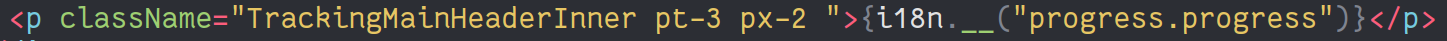
\includegraphics[width = 15cm]{src/public/oppar/translationcall.png}\\
Kuva \getImgCount. {} I18n käännösfunktiokutsu 
\medskip


% emt onko incoherent

I18n kirjasto tukee montaa käännöstiedosto formaattia, mutta sovellukseen valittiin JSON tiedostomuoto.
Kuvassa \nextImageCount{} on progressio sivun suomenkieliset käännökset ja kuvassa {\the\numexpr \theimgCounter + 2 } on saman sivun englannin kieliset käännökset.
Jokaisella sovelluksen sivulla on oma objekti, joka sisältää sen sivun julkisen tekstin. 
Avaimet tekstille on valmiiksi määritellyt merkkijonot, jotka kuvaavat käännöksen tarkoitusta.
Kun käyttäjä vaihtaa halutun kielen i18n osoittaa toiseen käännöstiedostoon, 
jossa on samat avaimet käännöksille, mutta arvot ovat vaihtuneet kyseisen kielen käännöksiin.
\medskip


\bigskip
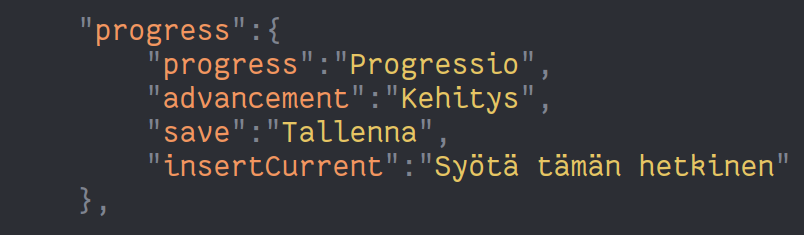
\includegraphics[width = 15cm]{src/public/oppar/translationfile.png}\\
Kuva \getImgCount. {} Progressiosivun suomenkielinen käännöstiedosto 
\medskip


\bigskip
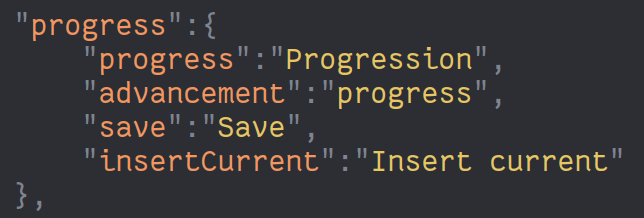
\includegraphics[width = 15cm]{src/public/oppar/translationfileEng.png}\\
Kuva \getImgCount {}. Progressiosivun englanninkielinen käännöstiedosto
\medskip




\subsection{Käyttöliittymä kielenvaihamiselle}

%lisäsin sivulle, tosin kun sivulle on lisätty

Sovellukseen on myös lisätty kuvan \nextImageCount{} laskuvalikko kielen vaihtamiselle. 
Kielet kuvataan lippuina laskuvalikossa,
sillä ne toimivat nopeina visuaalisina vihjeinä, jotka auttavat käyttäjiä tunnistamaan haluamansa kielen.
Laskuvalikko on näkyvissä sovelluksen kaikilla sivuilla, joten se on aina saatavilla.
\medskip



Laskuvalikon komponentti päivittää sovelluksen React root komponentin kun käyttäjä on vaihtanut kielen.
Tällöin varmistetaan että kaikki sivuilla oleva teksti vaihtuu oikeaan kieleen.
%jotain pikkusen lisää
\medskip


\bigskip

\includegraphics[]{src/public/locale_laskuvalikko.png}\\
Kuva \getImgCount {}. Kielen vaihto laskuvalikko













\newpage
\addPageOpfeat{src/op/feature.tex}{Uuden ominaisuuden lisäys} % ------------------------------- FEATURE ------------------------------- %










\newpage
\section{Yhteenveto}             % ------------------------------- YHTEENVETO ------------------------------- %


% mitä kaikkea pitää yhteenvetää

% pvopparimalli sanoo että tiivistelmään kuuluu
% kehityksen arviointi
% jatkotoimenpiteet
%
% itse tässä ei mainita että pitäisi tiivistää mitään mitä on itse käytännössä tehnyt
% mutta voisi kuitenkin mainita jutuista esim db backup jne




Opinnäytetyössä seurattiin projektin etenemistä ja kehittäjän oppimista seurantajakson ajan,
jolloin saatiin kattava yleiskuva projektin kehityksestä.
Lisäksi päiväkirja tarjoaa hyvän näkemyksen ammattilaisen päivittäisestä työstä ja tuo esiin rutiininomaiset ja monimutkaiset haasteet. 
Päiväkirja oli olennainen väline käytettyjen teknologioiden opiskeluun,
ja sen avulla voin ymmärtää perusteellisemmin niiden soveltamista, vahvuuksia ja rajoituksia. 
Päiväkirja dokumentoi päivittäiset kokemukset ja pohdinnat,
joten se mahdollisti yksityiskohtaisen analyysin, joka paransi merkittävästi oppimisprosessiani.
\medskip





Työskentely uusien teknologioiden parissa on antanut minulle mahdollisuuden syventyä omaan oppimisprosessiini, 
mikä on parantanut teknisiä taitojani.
Lisäksi olen parantanut sosiaalisia taitojani kommunikoidessani muiden projektin jäsenten kanssa.
Vuorovaikutus on parantanut kykyäni tehdä tehokasta yhteistyötä,
ilmaista ajatukseni selkeästi ja rakentaa vahvoja ammatillisia suhteita,
jotka kaikki ovat välttämättömiä menestyksen kannalta. \\
\medskip


% sanoja itsenäisestä työskentelystä ja sosiaalisista taidoista.

Ammattilaisympäristössä työskentelystä saatu kokemus on antanut minulle useita taitoja ja näkemyksiä, 
joista on hyötyä tulevaisuudessa.
Ominaisuuksien toteuttamisprosessi on antanut minulle käytännön kokemusta ohjelmistosuunnittelusta. 
Lisäksi olen oppinut selviytymään monimutkaisista teknisistä haasteista,
optimoimaan suorituskykyä ja varmistamaan ohjelmiston skaalautuvuuden ja ylläpidettävyyden.
Tämä kokemus ei ole ainoastaan lisännyt teknisiä taitojani vaan myös parantanut ongelmanratkaisukykyäni ja yksityiskohtien huomioimista, 
mikä valmistaa minua tuleviin tehtäviin ohjelmistokehityksen ja -tekniikan alalla.

\medskip



% miten käytän tätä mitä opin

%
Työharjoittelusta ja oppimispäiväkirjan kirjoittamisesta saamani kokemus tulee auttamaan minua tulevaisuudessa.
Työharjoittelu tarjosi käytännön kokemusta todellisista ammatillisista ympäristöistä,
minkä ansiosta pystyin soveltamaan koulussa opittuja teoriatietoa todellisiin projekteihin ja kehittämään kriittisiä taitoja 
ongelmanratkaisussa ja tiimityössä.
Samalla oppimispäiväkirjan pitäminen helpotti kokemusteni jatkuvaa pohdintaa,
minkä ansiosta pystyin seuraamaan edistymistäni,
tunnistamaan parannuskohteita ja syventämään ymmärrystäni käytetyistä tekniikoista ja menetelmistä.
Yhdessä nämä kokemukset ovat parantaneet ammatillisia taitojani ja toimivat vankkana perustana tuleville urapyrkimyksilleni.
\medskip













% this is not what is wanted to be written in the yhteenvet
\iffalse

Käännökset/lokalisaatio meni hyvin ja sovellus on nyt parempi.
Käännöksien käyttöönotto meni ongelmitta.
itse sisällön käännös oli tehty henkilö käännöksellä joten se on hyvänlaatuinen.
%
Sovelluksella on nyt keskitetty tiedostosijainti missä, kaikki sovelluksen julkipuolen teksti sijaitsee.
Käännökset on eroteltu niille kuuluville sivuille, joten niiden etsiminen on helppoa.
Keskitetty tekstipankki auttaa sovelluksen kehittämisessä tulevaisuudessa,
sillä jos haluaa etsiä tekstiä sivuilta ei tarvitse alkaa etsimään komponentteja missä teksti sijaitsee,
vaan etsiä se käännöstiedostosta.
%
Käännöksiin käytetty I18n kirjastossa oli kattava dokumentaatio, joka auttoi käännöksien toteuttamisessa.
%more??
\medskip



Uusi ominaisuus toimi käyttöönoton jälkeen ja kaikki käyttäjät saivat ominaisuuden käyttöön.
Käyttäjät pystyi tallentamaan useamman mitattavan arvon ja näkemään tulokset kaaviossa. %vähän repeat 
%reword this
Viikko ominaisuuden käyttöönoton jälkeen testiryhmältä ei tullut palautetta, että ominaisuus ei olisi toiminut.
%
käyttöliittymästän toiminnasta tai sen ulkonäöstä ei myöskään tullut palautetta sen käyttöönoton jälkeen.
%
Käyttäjä profiilin skeeman migratointi meni onglemitta.
Riskit käyttäjien skeeman migraation epäonnistummisessa olisi voinut välttää ottamalla varmuuskopio tietokannasta ennen migraatiota.
\medskip



opin käyttämään projektissa käytettyjä teknologioita.
opin tekemään töitä ammatillisessa työympäristössä.
opin lisää web alustoista ja niiden kanssa töiden tekemisestä.
%jotain oikeaa concrete mainintaa tästä opparin tavaoitteesta
\medskip


alustan kanssa työskentely oli jees.
isomman koodi pohjan kanssa työskentely jossa muut ihmiset ovat olleet mukana oli hyvä kokemus.
%jotain sanoja alustan kanssa työskentelemästä ja starttaamo työympäristöstä
\medskip

\fi








\newpage
% we need some way to manually override an item when it looks like shit

% i thin we need to make our own @ thing then use that for htings that look like shit
% though i dont thik we need the hfill thing in the first place but whattever that is problem for another day


%(korjaa outo spacing)
\bibliographystyle{labCitations} % ------------------------------- LÄHTEET ------------------------------- %
\bibliography{./src/op/citations}


%https://libguides.eur.nl/overleaf/bibliographies-and-citing
%https://tex.stackexchange.com/questions/51434/biblatex-citation-order
% i want to do citations like this but if there is problem with the format then must do manually or... write own system





\section*{Liitteet}               % ------------------------------- Liitteet ------------------------------- %

Oppimispäiväkirja



% if we compiled the pv at the same time it would take too long
\includepdf[pages=-]{output/paivakirja.pdf}



\end{document}
